
\def\INDEXSET#1{\mathit{#1}_{[P]}}
\def\baselinestretch{1.5}

\section{Construction of Partial Trees}
\label{sec:construction}

Since the structure of partial tree is quite different from ordinary XML trees,
especially the pre-path, ordinary XML parsing algorithms, in turn, do not work
for the construction of partial tree. The difference mainly lies in two aspects.
First, an XML document can generate only a single XML tree. While in case of
partial tree, the number of XML trees could be many, which is determined by the
number of chunks. However, we cannot simply construct an partial tree from a
chunk. This is caused by the second reason that the pre-path of a partial tree
is missing in the corresponding chunk.

For constructing the pre-path, it is important that a partial tree that
corresponds to a chunk is the minimum subgraph. It should satisfy the following
three conditions:

(1) the subgraph is connected (This means the subgraph is a tree.);

(2) each node in the chunk is in the subgraph, and

(3) the root of the original XML tree is in the subgraph.

For an intuitive grasp, we use the following XML document as the running
example.

\begin{quote}\tt\small
<A><B><C><E></E></C><D></D></B><E></E><B><B><D><E>\\
</E></D><C></C></B><C><E></E></C><D><E></E></D></B>\\
<E><D></D></E><B><D></D><C></C></B><B></B></A>\\
\end{quote}

From the document, we can construct an XML tree as shown in Fig.~\ref{fig:tree}.
We number all the nodes of the tree in a prefix order for identification.



To construct partial trees from the document, we first split it into five chunks
as listed below.

 chunk$_0$: \texttt{ <A><B><C><E></E></C><D></D></B>}

 chunk$_1$: \texttt{ <E></E><B><B><D><E></E></D>}

 chunk$_2$: \texttt{ <C></C></B><C><E></E></C><D>}

 chunk$_3$: \texttt{ <E></E></D></B><E><D></D></E>}

 chunk$_4$: \texttt{ <B><D></D><C></C></B><B></B></A> }


\begin{figure*}[t]
	\centering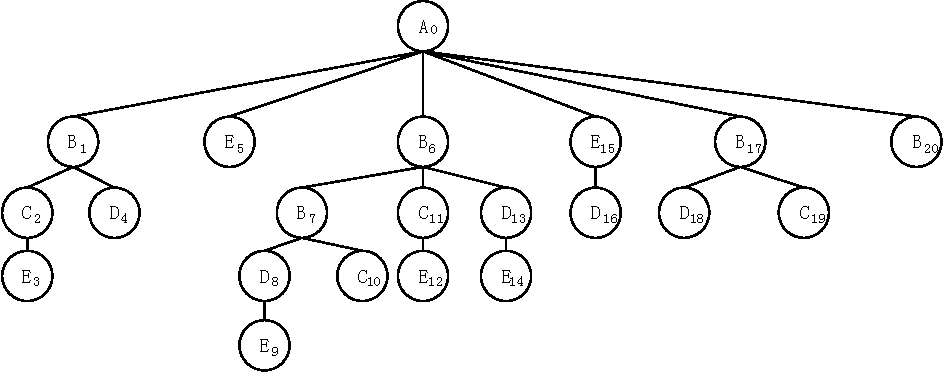
\includegraphics[scale=.9]{partialtree/figures/fromWord-5.pdf}
	\caption{an XML tree from the given XML string}
	\label{fig:tree}
	
	\centering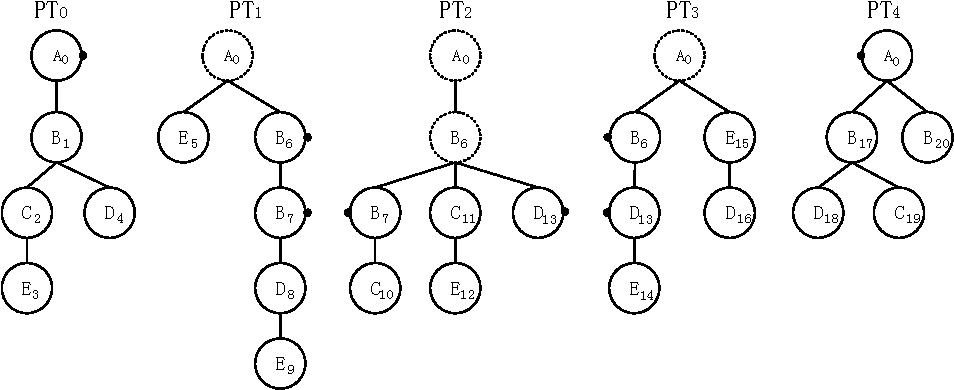
\includegraphics[scale=.9]{partialtree/figures/fromWord-7.pdf}
	\caption{Partial trees from the given XML string.}
	\label{fig:partialtree2}
\end{figure*}

We can construct a parital tree from each chunk, i.e. chunk$_i$ makes a partial
tree PT$_i$, as shown in Figure~\ref{fig:partialtree2}.

In the following section, we introduce our partial tree construction algorithm
with the example. Our algorithm is a three-phase algorithm. In the first phase,
we construct mutiple sets of subtrees that have some open nodes from parsing
chunks of the input XML document. Second, we compute pre-path for each list of
subtrees with all the open nodes. Last, we add pre-paths to the corresponding
list of subtrees to complete the partial tree construction. We will give deailed
introduction to the three-phase construction algorithm of partial tree.
Furthermore, to server the query algorithm, we also introduce the statistics
information of open nodes, called ranges of open nodes. With such information,
we can easily access open nodes of the same node and synchronize the query
results among partial trees.

\subsection{Construction of Subtrees From Parsing XML Chunks}

As introduced previously, a partial tree is constructed from parsing an input
XML chunk, which is a substring generated from splitting the XML document. We
design an algorithm that parses the input XML string into a similar tree by
using an iterative function with a stack, which is similar to ordinary XML
parsing algorithms.

First, after splitting an XML document, we deal with nodes with missing tags.
During parsing, we push start tags onto the stack. When we meet an end tag, we
pop a last start tag to merge a closed node. However, as a result of splitting,
some nodes miss their matching tags. In this case, we mark it left-open or
right-open based on which tag (either start tag or end tag) is missing. Then, we
add them onto the subtrees in the same way as we add closed nodes.

We also need to handle the case when the split position falls inside a tag and
thus splits the tag into two halves. In this case, we simply merge the split
tags. Because there are at most two split tags on a partial tree, the time taken
for merging them is negligible.

One or more subtrees can be constructed from a single chunk. For example, we
can construct nine subtrees from parsing the five chunks above as shown in
Fig.~\ref{fig:partialtree-notfinished}. Chunk$_0$ and chunk$_4$ have only one
subtree while chunk$_2$ has three subtrees. After the parsing phase, these
subtrees are used for pre-path computation.

\begin{figure*}[t]
	\centering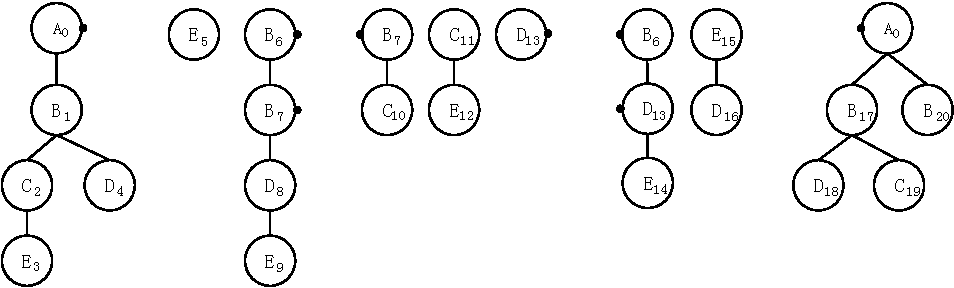
\includegraphics[]{partialtree/figures/fromWord-6.pdf}
	\caption{Subtrees from parsing chunks}
	\label{fig:partialtree-notfinished}
\end{figure*}


\subsection{Pre-path Computation}

The key idea of computing the pre-path for each partial tree is to make use
of open nodes. This is because the missing parent and ancestor nodes are caused
by splitting those nodes. Therefore, the information needed for creating the
pre-paths lies in them.

Algorithm 0 outlines the pseudo codes for computing pre-path. Since one chunk
may generate more than one subtrees, the input is a list of subtree lists. The
length of the list is equal to the number of partial trees, i.e. one chunk makes
one list of subtree, thus representing the length as $P$.

Algorithm 0 has three phases. In the first phase, it selects all the left-open
nodes into $LLS$ and all the right-open nodes into $RLS$ (line 2-4). $LLS_{[P]}$
collects the left-open nodes of the $p$th partial tree, likewise we have
$RLS_{[P]}$. Note that the nodes in $LLS_{[P]}$ or $RLS_{[P]}$ are arranged in
order from the root to leaves. For example, in Table~\ref{table:opennodes}, we
select all the open nodes and add them to corresponding lists.

{
	\setstretch{1.5}
\begin{figure}[!t]
 	\centering
 	\label{fig:ppalgorithm}
 	\begin{tabular}{l}
 		\hline
 		\hline
 		\makebox[.95\linewidth][l]{\textbf{Algorithm 0} \textsc{GetPrepath}($\mathit{STS}$)} \\
 		\hline
 		\textbf{Input}: $\mathit{STS}$: a list of subtree lists \\
 		\textbf{Output}: an list of partial trees\\
 		\makebox[1em][r]{1:}\hspace{1 mm} /* open nodes in LLS or RLS are arranged in top-bottom order */\\
 		\makebox[1em][r]{2:}\hspace{1 mm} \textbf{for all} $p \in [0, P)$ \textbf{do} \\
 		\makebox[1em][r]{3:}\hspace{4 mm} $\INDEXSETL{LLS} \leftarrow \mathit{SelectLeftOpenNodes}(\INDEXSETL{STS})$\\
 		\makebox[1em][r]{4:}\hspace{4 mm} $\INDEXSETL{RLS} \leftarrow \mathit{SelectRightOpenNodes}(\INDEXSETL{STS})$\\

 		\makebox[1em][r]{5:}\hspace{1 mm} /* Prepath-computation and collecting matching nodes */\\
 		\makebox[1em][r]{6:}\hspace{1 mm} $AuxList \leftarrow []$ \\
 		\makebox[1em][r]{7:}\hspace{1 mm} \textbf{for} $ p \in [0, P-1) $ \textbf{do}\\
 		\makebox[1em][r]{8:}\hspace{4 mm} $AuxList.\mathit{AppendToHead}(\INDEXSETL{RLS})$\\
 		\makebox[1em][r]{9:}\hspace{4 mm} $AuxList.\mathit{RemoveLast}(LLS_{[p+1]}.\mathit{Size}()) $\\
 		\makebox[1em][r]{10:}\hspace{4 mm} $ PPS_{[p+1]}\leftarrow AuxList$ \\

 		\makebox[1em][r]{11:}\hspace{1 mm}  /* Add pre-nodes to subtrees */ \\
 		\makebox[1em][r]{12:}\hspace{1 mm} $PTS \leftarrow []$ \\
 		\makebox[1em][r]{13:}\hspace{1 mm} \textbf{for} $ p \in [0, P) $ \textbf{do}\\
 		\makebox[1em][r]{14:}\hspace{4 mm} \textbf{for} $ i \in [0, PPS_{[p]}.Size() - 1)$ \textbf{do} \\
 		\makebox[1em][r]{15:}\hspace{8 mm}   $PPS_{[p][i]}.children.$Add$(PPS_{[p][i+1]})$ \\
  		\makebox[1em][r]{16:}\hspace{4 mm} $PPS_{[p]}.last.children.$Add$(\INDEXSETL{STS})$ \\
 		\makebox[1em][r]{17:}\hspace{4 mm}   $\INDEXSETL{PTS} \leftarrow PPS_{[p][0]}$ \\
 		\makebox[1em][r]{18:}\hspace{1 mm} \textbf{return} \emph{PTS} \\
 		\hline
 	\end{tabular}
 \end{figure}
}

In the second phase, we perform the pre-path computation. Once we split an XML
document from a position inside the document, the two partial trees created from
the splitting have the same number of open nodes on the splitting side. Given
two consecutive partial trees, the number of the right-open nodes of the left
partial tree is the same as the number of the left-open nodes of the right
partial tree. This is a very important feature and we exploit it for computing
the pre-paths of partial trees.

In the algorithm, we first add the $p$th $RLS$ to the head of an auxiliary list
$AuxList$ (line 8), and then we remove the same number of nodes as the number of
$(p-1)$th $LLS$ (line 9). Last, we keep the nodes in the $AuxList$ to the
$(p+1)$th $PPS$, which holds the pre-nodes for each partial tree.
Table~\ref{table:tempresult} shows the results of pre-path computation for the
given example.

{
\setstretch{1.5}
\begin{table}[t]
	\caption{Open node lists}
	\label{table:opennodes}
	\centering
	\begin{tabular}{c|cc}
		\hline
		& Left-open nodes	& Right-open nodes \\
		\hline
		pt$_0$	& []			& [A$_0$] \\
		pt$_1$	& []			& [B$_6$, B$_7$] \\
		pt$_2$	& [B$_7$]			& [D$_1$$_3$] \\
		pt$_3$	& [B$_6$, D$_1$$_3$]		& [] \\
		pt$_4$	& [A$_0$]			& [] \\
		\hline
	\end{tabular}

	\caption{Results of pre-path computation in AUX}
	\label{table:tempresult}
	\centering
	\begin{tabular}{c|ccc}
		\hline
		& Left-open nodes	& Right-open nodes & $AUX$\\
		\hline
		pt$_0$	& []			& [A$_0$]  & []\\
		pt$_1$	& []			& [B$_6$, B$_7$] & [A$_0$] \\
		pt$_2$	& [B$_7$]			& [D13] &[A$_0$,B$_6$]\\
		pt$_3$	& [B$_7$, D$_1$$_3$]		& []  & [A$_0$]\\
		pt$_4$	& [A$_0$]			& [] &[]\\
		\hline
	\end{tabular}
\end{table}
}

In last phase, we add the resultant pre-nodes to the corresponding partial trees
and copy the nodes from $PPS_{[p]}$ to $PTS_{[p]}$ as the results for output.
Because the pre-nodes in the pre-path are also open nodes, we list all open
nodes for each partial trees in Table~\ref{table:allopennodes}. Then, the
pre-path computation is complete. For the given example, we obtain the partial
trees as shown in Fig.~\ref{fig:partialtree2}.


\subsection{Creation of Ranges of Open Nodes}
\label{sec:ranges}

Once an XML node is split, it generates two or more open nodes of the same node
in consecutive partial trees. For example, as we can see in
Fig.~\ref{fig:partialtree2}, \Nr{B}{6} on pt$_1$, \Np{B}{6} on pt$_2$, and
\Nl{B}{6}  on pt$_3$ are created from the same node \Nc{B}{6}. For locating the
open nodes of the same node,  which are distrubted in different partial trees,
we use two integers \textit{start} and \textit{end} for an open node. With these
two integers, we can know the partial trees that have matching nodes of the same
open node. Note that after adding nodes to a partial tree, the open nodes from
the same node also have the same depth. Therefore, we can locate all the
matching nodes to set \textit{start} and \textit{end} for each open node. After
computation, we obtain the ranges of nodes as shown in
Table~\ref{table:rangesresult}.

{
	\setstretch{1.5}
\begin{table}[t]
		\caption{All open nodes}
	\label{table:allopennodes}
	\centering
	\begin{tabular}{c|cc}
		\hline
		& Left-open nodes	& Right-open nodes \\
		\hline
		pt$_0$	& []						& [A$_0$] \\
		pt$_1$	& [A$_0$]					& [A$_0$, B$_6$, B$_7$] \\
		pt$_2$	& [A$_0$, B$_6$, B$_7$]		& [A$_0$, B$_6$, D$_1$$_3$] \\
		pt$_3$	& [A$_0$, B$_6$, D$_1$$_3$]	& [A$_0$] \\
		pt$_4$	& [A$_0$]					& [] \\
		\hline
	\end{tabular}

	\caption{Open node lists with ranges}
	\label{table:rangesresult}
	\centering
	\begin{tabular}{c|cc}
		\hline
		& Left open nodes	& Right open nodes \\
		\hline
		pt$_0$	& []	& [A$_0$(0,4)] \\
		pt$_1$	& [A$_0$(0,4)]	& [A$_0$(0,4), B$_6$(1,3), B$_7$(1,2)] \\
		pt$_2$	& [A$_0$(0,4), B$_6$(1,3), B$_7$(1,2)]	& [A$_0$(0,4), B$_6$(1,3), D$_1$$_3$(2,3)] \\
		pt$_3$	& [A$_0$(0,4), B$_6$(1,3), D$_1$$_3$(2,3)]	& [A$_0$(0,4)] \\
		pt$_4$	& [A$_0$(0,4)]	& [] \\
		\hline
	\end{tabular}
\end{table}
}

By using these ranges, we can esaily establish the partial trees for the
matching nodes of the same node. For example, the range of A$_0$ is (0, 4), that
means we can locate the same nodes of \Nc{A}{0} from pt$_0$ to pt$_4$. As we can
see, there are \Nr{A}{0}, \Np{A}{0}, \Np{A}{0}, \Np{A}{0}, and \Nr{A}{0} on
pt$_0$ to pt$_4$, respectively.
